\documentclass[10pt]{article}

\usepackage[hmarginratio=1:1,top=32mm,columnsep=20pt]{geometry}                 \usepackage{booktabs}     	
\usepackage{graphicx}
\usepackage{subcaption}
\usepackage[backend=bibtex,sorting=none]{biblatex}
\usepackage{hyperref}
\hypersetup{colorlinks=false,
            urlcolor=blue}
	    
\bibliography{references}

\title{Healthcare Data Lake}

\author{
	\textsc{Kendal, Joseph}\\
	\normalsize University of Bristol\\
	\texttt{jk17246@bristol.ac.uk}
	
	\and
	
	\textsc{Sherred, Jago}\\
	\normalsize University of Bristol\\
	\texttt{j.sherred.2019@bristol.ac.uk}
	
	\and
	
	\textsc{Benson, Luke}\\
	\normalsize University of Bristol\\
	\texttt{wr19606@bristol.ac.uk}
	
	\and
	
	\textsc{Liu, Anna}\\
	\normalsize University of Bristol\\
	\texttt{gf19916@bristol.ac.uk}
	
	\and
	
	\textsc{Cismaru, Armand}\\
	\normalsize University of Bristol\\
	\texttt{fz19792@bristol.ac.uk}
}


\begin{document}

\maketitle    


\begin{abstract}

Digital healthcare provided by the NHS in England typically operates in silos. GPs have electronic systems to manage patient care which are distinct from hospital systems which are distinct from the ambulance service, 111, mental health services etc. Each data owner has a wealth of data that, if combined, would generate a more valuable resource than it does in isolation. While there are solutions to integrate this data for direct care purposes, there is no centralised solution to use this data to inform future care or service provisioning. This project is designed to explore the benefits of cloud technologies to produce a prototype secure, scalable health data storage platform that can underpin local healthcare analytics.

\end{abstract}

\section{Overview}
%TODO%

\subsection{Client}
Dr. Philip D Harfield, Health Data Scientist (Informatics) at NIHR Bristol Biomedical Research Centre, University of Bristol.
\subsection{Domain}
The domain of our Healthcare Data Lake project is the Healthcare Analytics Environment team who will design, implement and test a set
of candidate cloud-hosted analytics environments that provide sufficient functionality while also maintaining a secure data environment.
\\
The overall domain of the three teams is NHS Healthier Together Sustainability Transformation Partnership Bristol, North Somerset, and South Gloucestershire (BNSSG) \& Bristol Biomedical Research Centre, University of Bristol Medical School.
\subsection{Project}
The project entails combining a wealth of data from data owners(GPs Patient data, ambulance services, 111, mental health services .etc) into a data lake. This will be used to inform clinical decisions making by providing more advanced insights into the longitudinal health of the patient on arrival and understand the merits of previous clinic decisions taken.
\\
The project will explore the benefits of cloud technologies and produce a prototype secure, scalable health data storage platforms that can underpin local healthcare analytics.
\\
The project is one of three designed an end-to-end proof of concept to the local NHS. We will be working alongside the "Healthcare Data Visualisation" and "Healthcare Analytics Environment" teams. 
\subsection{Vision}
The Healthcare Data Lake Project is envisioning a future integrated data storage solution, one that is scalable and portable, while using the latest cloud-based technologies. Starting with a prototype, the final scope is to create, alongside the Simulation and Analytics Projects, a system that is going to change how data is handled and used in the healthcare system. There is the real possibility that this three projects will represent the cornerstone of a future solution used and developed extensively by the NHS, which will bring immediate aid to the average medical worker and improve the quality of the service provided to the patients.



\section{Stakeholder and Requirements
Analysis}\label{stakeholder-and-requirements-analysis}

\subsection{Primary Stakeholder and User
Story}\label{primary-stakeholder-and-user-story}

Philip Harfield at Bristol, North Somerset and South Gloucestershire CCG
(BNSSG). Philip Harfield is our client, and this software is being
developed for him at BNSSG. The user story for this stakeholder is that
BNSSG require a piece of software that can be used to allow long-term
healthcare data analytics from multiple data sources to inform clinical
and strategic decisions. The reason for this is understanding the
longitudinal health of a patient allows understanding of the merits of
previous clinical decisions taken. In addition it can be used to inform
strategic commissioning decisions using data on how effective services
offered to patients have been.

\subsubsection{Flow steps}\label{flow-steps}

Considering the user story above, we can breakdown the story into a
sequence of steps of user flow.

\begin{enumerate}
\def\labelenumi{\arabic{enumi}.}
\itemsep1pt\parskip0pt\parsep0pt
\item
Local healthcare service authenticates their identity.
\item	
	Local healthcare service provides information to the data lake.
\item
  Data is transformed and loaded into the data lake.
\item
  The data is catalogued in the data lake and stored in structured data
  marts as required.
\item
  The data lake allows access to a data analytics environment.
\item
  An analytics environment can run queries on the data lake and report
  results to analytics environment.
\item
  Clinical and strategic decisions can be taken based on analysis.
\end{enumerate}

We can also identify alternative or exceptional flows. 
\subparagraph{Exceptional Flow:}

\begin{enumerate}
\def\labelenumi{\arabic{enumi}.}
\itemsep1pt\parskip0pt\parsep0pt
\item	
Local healthcare service is authenticated.
\item
  Local healthcare services provide data to the data lake.
\item
  Data is not provided in an acceptable format to the API.
\item
  The healthcare service receives an error message to provide data in
  standard format.
\end{enumerate}

\subparagraph{Exceptional Flow:} 	
\begin{enumerate}	
	\def\labelenumi{\arabic{enumi}.}	
	\itemsep1pt\parskip0pt\parsep0pt	
	\item Local healthcare service fails to be	
	authenticated.	
	\item The service receives an error message to provide valid	
	credentials.	
	\item Incoming data is not accepted.	
\end{enumerate}

\subsubsection{Atomic Requirements}\label{atomic-requirements}

We can breakdown these steps into atomic requirements of the software.

\begin{enumerate}
\def\labelenumi{\arabic{enumi}.}
\itemsep1pt\parskip0pt\parsep0pt
\item	
An identity authentication process provides healthcare providers with	
credentials to supply data to the API.
\item
  An API takes in data from local healthcare providers as a HL7 FHIR
  message. We have chosen HL7 FHIR as it is the
  \href{https://digital.nhs.uk/services/fhir-uk-core}{UK   standard
  for
 transferring healthcare messages.}
\item
  These data messages are stored in a cloud solution in a well
  structured data model.
\item
  Ingested data is catalogued.
\item
  An ETL tool is used to curate data marts.
\item
  These data marts can be queried by the analytics environment.
\end{enumerate}

There are also additional requirements specified for the software:

\begin{enumerate}
\def\labelenumi{\arabic{enumi}.}
\itemsep1pt\parskip0pt\parsep0pt
\item
  Medical data is to be stored independently from pseudonymised patient
  identifiers.
\item
  Provide a user console to monitor automated ETL jobs.
\item
  Provide full audit trails.
\end{enumerate}

\subsection{Additional stakeholders and User
Stories}\label{additional-stakeholders-and-user-stories}

This software will provide services to a number of local healthcare
organisations such as NHS trusts and the Healthier Together STP and such
all these additional users are secondary stakeholders to this project.
These organisations will need to be able to provide healthcare
information to the software which will need to be able to load and store
the data for future analysis.

\subsubsection{Flow Steps}\label{flow-steps-1}

Considering the user story above, we can breakdown the story into a
sequence of steps of user flow.

\begin{enumerate}
\def\labelenumi{\arabic{enumi}.}
\itemsep1pt\parskip0pt\parsep0pt
\item
  Healthcare provider (e.g.~Hospital Trust) provide data to the data
  lake by a HL7 FHIR message.
\item
  The data is stored in the data lake.
\end{enumerate}

We can also consider the stakeholder of a developer and their user story	
of accessing a user control to monitor automated ETL jobs to identify	
live support issues.	

\subparagraph{Flow Steps}

This can be broken into the following user flow.	

\begin{enumerate}	
	\def\labelenumi{\arabic{enumi}.}	
	\itemsep1pt\parskip0pt\parsep0pt	
	\item	
	Developer authenticates identity.	
	\item	
	Developer accesses user interface which logs all automated ETL jobs	
	carried out on the data lake.	
	\item	
	Developer can use information to identify issues and provide support.	
\end{enumerate}

\newpage
\section{Personal Data, Privacy, Security and Ethics Management}
\subsection{GDPR}
The data lake solution developed by the “Healthcare Data Lake” project team is an integrating part of the larger prototype system, alongside "Healthcare Data Visualisation" and "Healthcare Analytics Environment" teams \emph{(section 1.3)}. The proposed system is going to be used in compliance with the \href{https://digital.nhs.uk/about-nhs-digital/our-work/keeping-patient-data-safe/gdpr}{\emph{NHS Digital GDPR}} compliance implementation and the liability for the personal data stored falls onto the respective primary stakeholder, Philip Harfield at Bristol, North Somerset and South Gloucestershire CCG (BNSSG) \emph{(section 2.1)}. The team developing the data lake infrastructure is responsible for creating a prototype secure, robust and scalable health data storage platform used for ingesting and interrogating patient’s data under the HL7 FHIR standard \emph{(section 4.1)}. As a client-specified requirement, medical data is going to be stored independently from the pseudonymised patient identifiers, thus protecting the identity and integrity of the patients whose data is stored in the data lake. The security of the data ingested as described in \emph {section 3.2} is aligned with the \href{https://digital.nhs.uk/about-nhs-digital/our-work/keeping-patient-data-safe/gdpr}{\emph{NHS Digital GDPR}} compliance and practice.

\subsection{Security}
\paragraph{}
The security requirements for this project are extremely high, and thus this implementation will enforce protections at every layer in the stack. The principle of least privilege (\texttt{PoLP}) applies with isolation and strong encryption to ensure data storage, access and communication is safeguarded from unauthorised processes in any event. The entire infrastructure is written in testable code to catch any mistakes before they hit production in the first place.
\paragraph{}
There will be no outbound (egress) communication from inside the data lake and the only inbound connection is data ingestion from the client API, which may in fact reside within a Virtual Private Network (\texttt{VPN}) to begin with rather than accessed over a public gateway. So that internet access is forbidden inside the Virtual Private Cloud (\texttt{VPC}) from our standpoint - so data exfiltration becomes challenging for an attacker that compromises any user account. All curated data marts are accessible via a peering link with the Data Analytics team who are responsible for the security of their environment in which they spawn their processes. All access to these will be logged and anomalies, violations and exceptions will be flagged for alerts and auditing. Furthermore, this  storage of curated data marts is in a private network separate from the rest of the data lake in any case. A comprehensive look at this architecture is included in \hyperref[sec:secure_access]{Section 4.5} and \hyperref[sec:network]{Section 4.6} of this paper. 

\subsection{Ethics}
Ethics pre-approval was applied for on 19 November 2020, 12:00 GMT. 
\\
\\
The data handled in the project is simulated patients data supplied by the Healthcare Data Simulation project. The Healthcare Lake project does not collect any data from any real person nor handles any consent, as the scope of the project is to create a secure infrastructure for storing patients data. \\ \\
In case of future development and testing with actual patients data, separate ethics approvals will be required, NHS REC review as it involves patients and governance approvals (e.g. Health Research Authority HRA). \emph{--client approvals and testing to be added--}

\newpage
\section{Architecture}
\subsection{Introduction}
We propose a modular, (cloud)platform-independent solution that offers high scalability and performance at a low cost for maintenance, development and deployment. The key to achieving this is leveraging the practises of infrastructure-as-code (IaC), serverless architectures and open standards. Therefore, development expense is focused on providing the most value, security and flexibility to the user.\\

\begin{figure}[h!]
	\centering
	\begin{subfigure}{0.25\linewidth}
		
\includegraphics[width=\linewidth]{images/Terraform.png}
	\end{subfigure}
	\begin{subfigure}{0.25\linewidth}
		
\includegraphics[width=\linewidth]{images/Serverless.png}
	\end{subfigure}
	\begin{subfigure}{0.25\linewidth}
		
\includegraphics[width=\linewidth]{images/OpenAPI.png}
	\end{subfigure}
\end{figure}

\paragraph{IaC}
By building infrastructure through extensible configuration files, we make it easy to build, test, secure, update and rollback versions of architecture which can combine multiple cloud or on-premise services. Terraform is an IaC framework that supports all major cloud providers in addition to self-hosted options such as Kubernetes. This makes it a popular choice for a modern infrastructure team that seeks to avoid vendor lock-in and easily protect the security of it with robust tests and auditing.

\begin{figure}[h!]
	\centering
	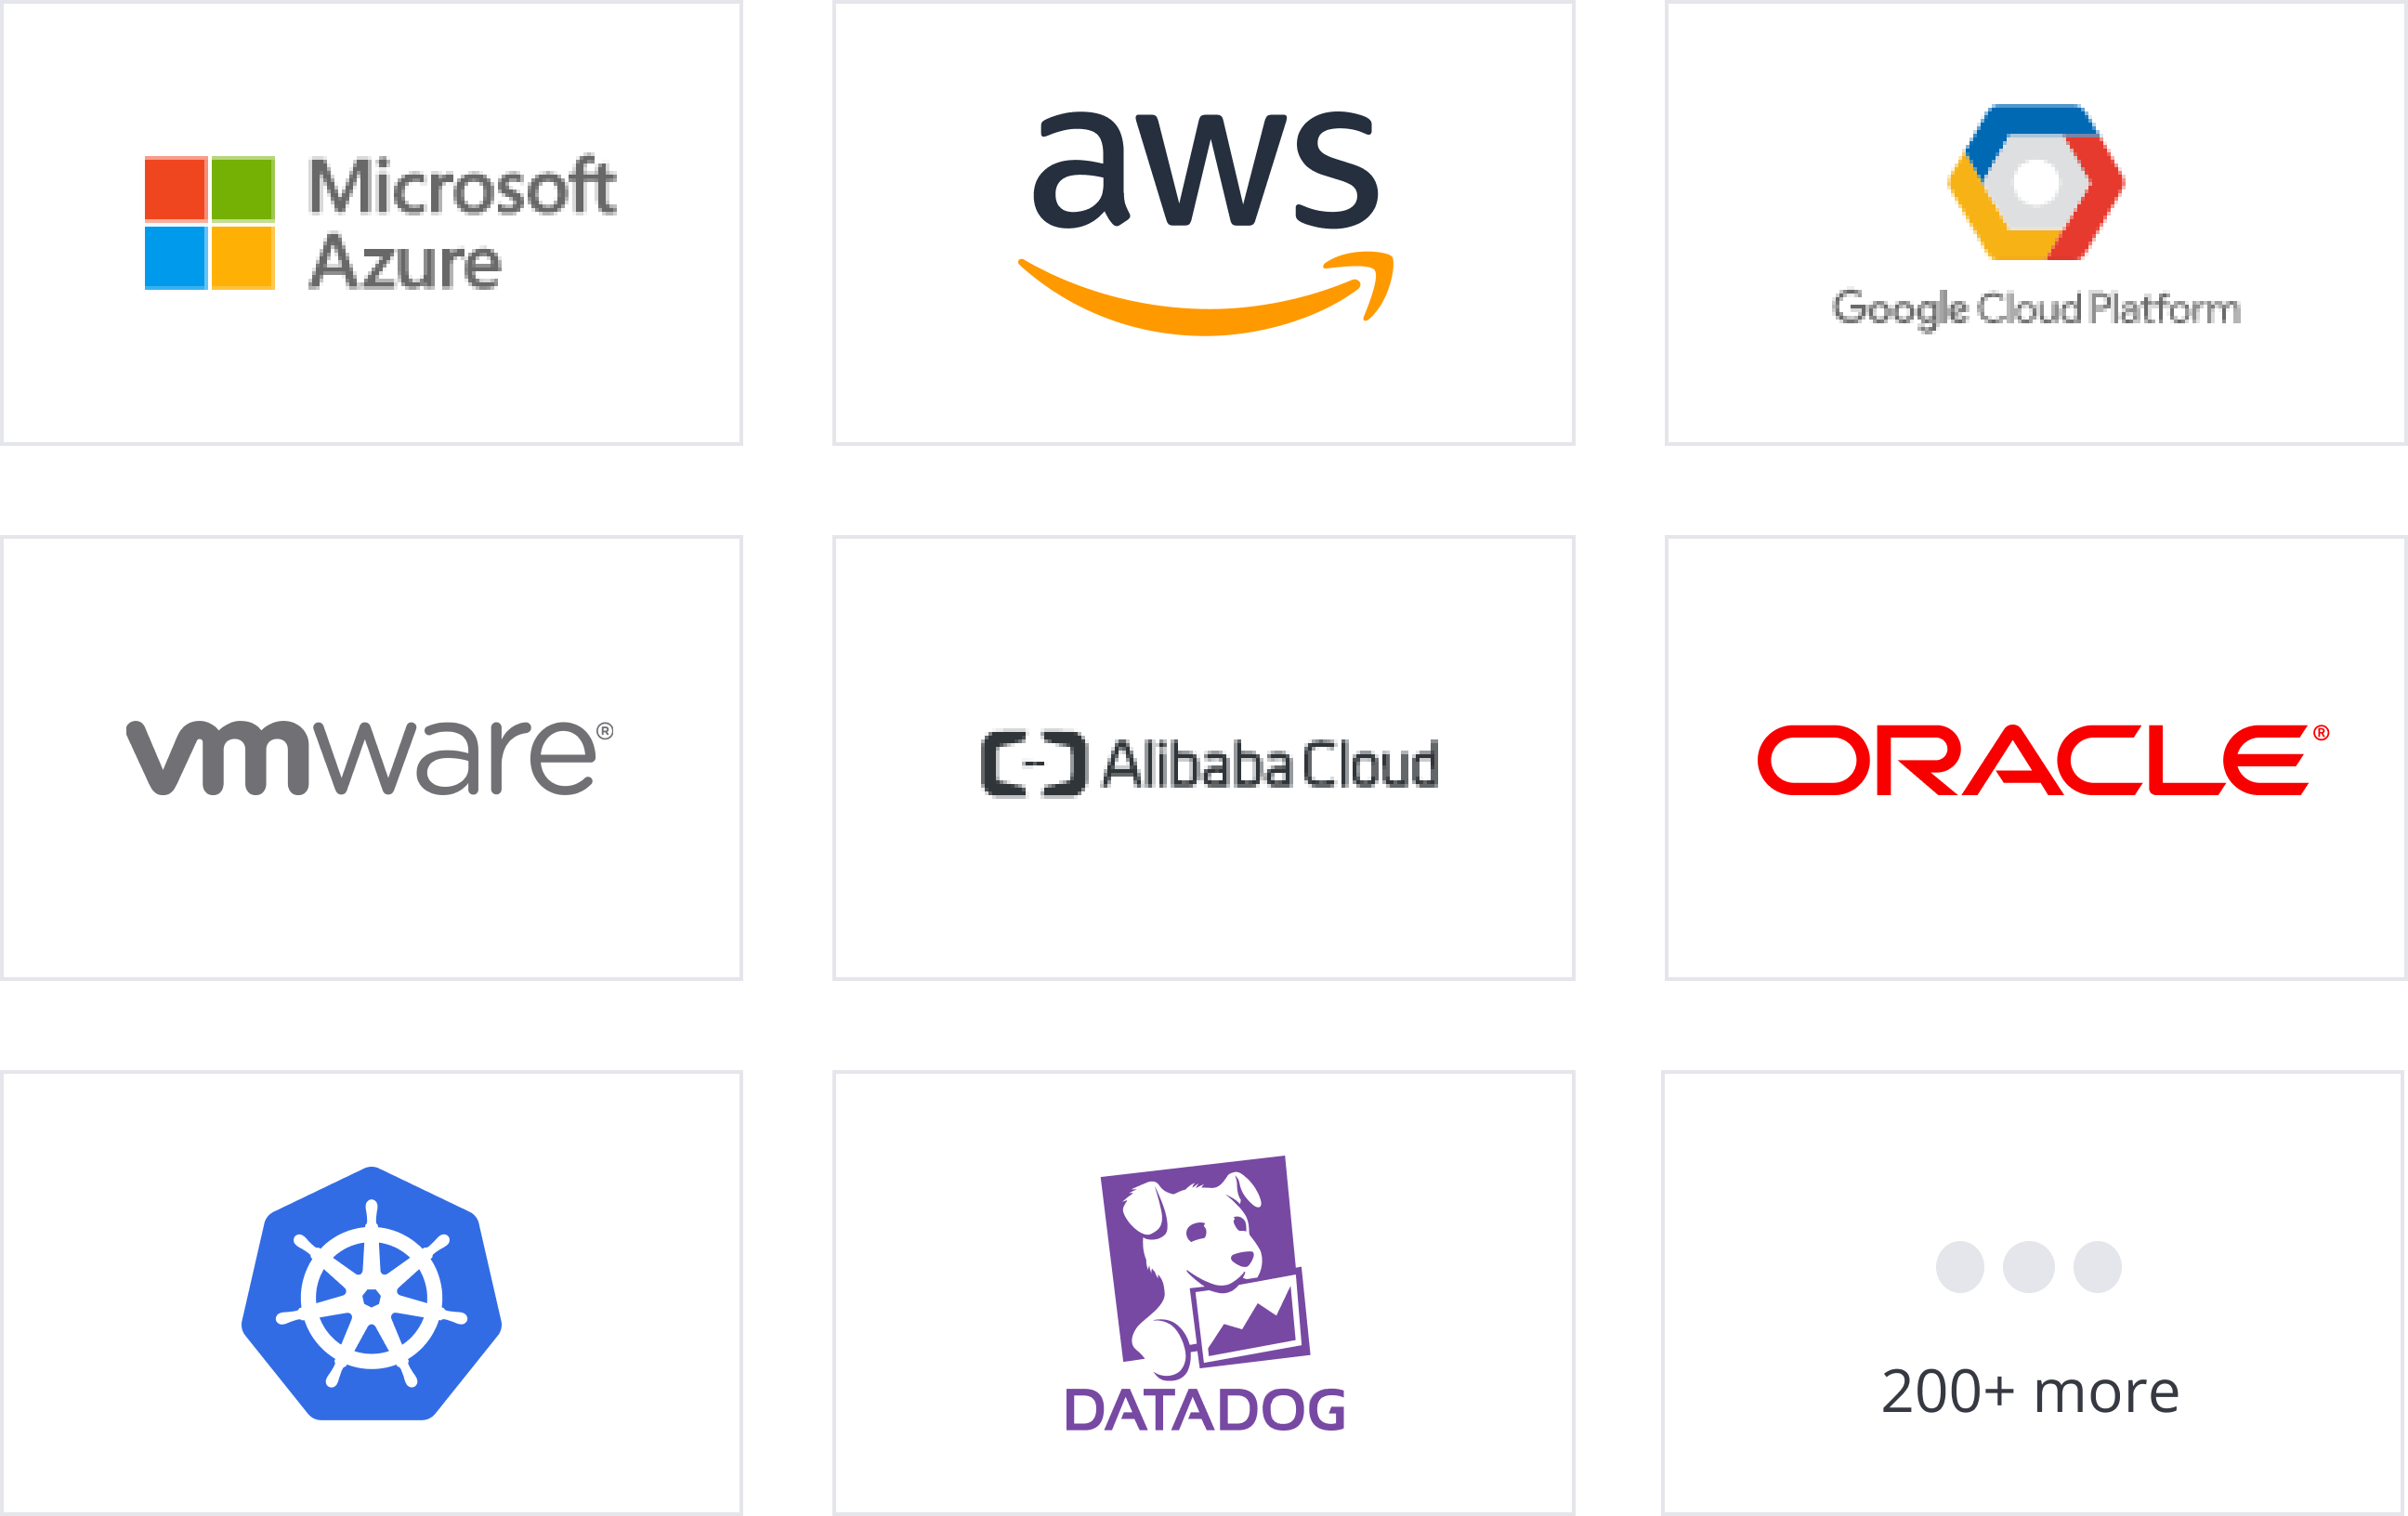
\includegraphics[width=0.55\linewidth]{images/TerraformProviders.png}	
\end{figure}

\paragraph{Serverless}
Serverless computing is a cloud computing execution model in which the cloud provider runs the server, and dynamically manages the allocation of machine resources. Pricing is based on the actual amount of resources consumed by an application, rather than on pre-purchased units of capacity \cite{serverless}. The benefits of this approach are the huge reduction in infrastructure and development expense. Engineers can focus on shipping their microservices and have secure, scalable infrastructure taken care of for them.
\\ \\
The Serverless Framework is also an example of IaC and provides developers with the ability to develop and deploy their serverless application to different cloud providers or simply Kubernetes (using \textbf{Knative}) if they wanted to run it on-premise or avoid code exposure to a cloud native service such as AWS Lambda or Google Cloud Functions.
\\ \\
This also provides quicker developer on-boarding and flexibility as a broad array of popular languages are supported. Given that the Function as a Service (\texttt{FaaS}) model is centred around the principles of loosely coupled microservices, this enables easy migration out of serverless architecture to a VM or container-based deployment. This may make sense in scenarios where there are cost savings to be made which typically applies to long-running, memory intensive tasks as opposed to short-lived and resource-light stateless services.


\paragraph{Open standards}
Open Standards allow people to share all kinds of data freely and with perfect fidelity. They prevent lock-in and other artificial barriers to interoperability, and promote choice between vendors and technology solutions. \cite{openstandards}

\subparagraph{OpenAPI}
The OpenAPI Specification (OAS) defines a standard, language-agnostic interface to RESTful APIs which allows both humans and computers to discover and understand the capabilities of the service without access to source code, documentation, or through network traffic inspection. When properly defined, a consumer can understand and interact with the remote service with a minimal amount of implementation logic. An OpenAPI definition can then be used by documentation generation tools to display the API, code generation tools to generate servers and clients in various programming languages, testing tools, and many other use cases. \cite{openapi}

\subparagraph{HL7 FHIR}
\textit{Fast Healthcare Interoperability Resources} (\texttt{FHIR}, pronounced "fire") is a standard describing data formats and elements (known as "resources") and an [API] for exchanging electronic health records (\texttt{EHR}). The standard was created by the Health Level Seven International (\texttt{HL7}) health-care standards organization. One of its goals is to facilitate interoperation between legacy health care systems, to make it easy to provide health care information to health care providers and individuals on a wide variety of devices from computers to tablets to cell phones, and to allow third-party application developers to provide medical applications which can be easily integrated into existing systems. \cite{fhir}

\subsection{Data ingestion}
The system will expose a RESTful endpoint for FHIR HL7 messages. It will not offer the full CRUD, only the Create and Update (when authorised). This accepts any structured or unstructured data when contained in a valid HL7 message. There is scope to build on this to add other data ingestion methods by building an API Facade that accepts other kinds of standards the client wants - such as medical IoT streaming data. This API will be accessible over a public gateway at first, with the intent to encourage developers to use a private link.
\subsubsection{API management}
\begin{minipage}{\textwidth}
	
\paragraph{Gateway}
AWS API Gateway automatically handles the caching, authentication, rate-limiting, routing, logging, validation, integration, scaling, versioning, mocking, documentation and usage plans of APIs defined with the OpenAPI specification. It also offers an affordable, flexible pricing model in exchange for handling these very challenging aspects of API development. Cutting time and cost, enabling teams to focus on shipping their code that actually matters.
\\

\begin{center}
	\centering
	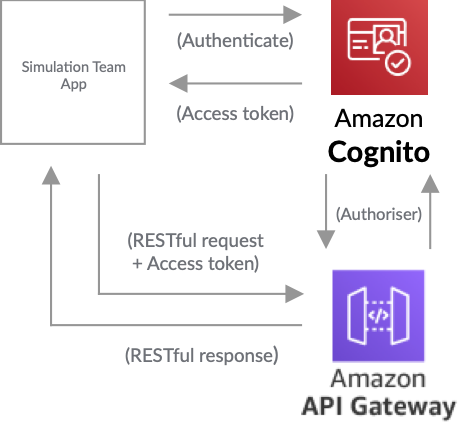
\includegraphics[width=0.4\linewidth]{images/APIGateway.png}
\end{center}

\paragraph{Authentication}
A healthcare service/simulation team app will first authenticate their identity with AWS Cognito which will supply the service with a secure access token. This token may be time-scoped and resource-scoped. The service can then use this token to access the API Gateway. This gateway uses strictly the latest version of TLS and requires the \texttt{Authorization} header to be set. This uses the AWS4-HMAC-SHA256 algorithm to calculate a signature for the secret key (access token). This is provided as a hexadecimal representation along with the other required parameters of access key (identity key) and requested resource. The Authorization header is added to all requests that contain the HL7 body for ingestion into the data lake. The API Gateway can then confirm with AWS Cognito to ensure the token is valid. If so then the HL7 FHIR message will be accepted.


\end{minipage}

\subsubsection{Microservices}
\begin{minipage}{\textwidth}
The API Gateway will forward requests to an AWS Lambda function that stores the data in S3, may send a notification using AWS Simple Notification Service (\texttt{SNS}) and writes metadata to the Glue catalogue. SNS notifications may trigger other microservices that prepare ETL jobs. These are yet to be scoped by the client but by default everything will be thrown into the lake where an EMR cluster can process.\\

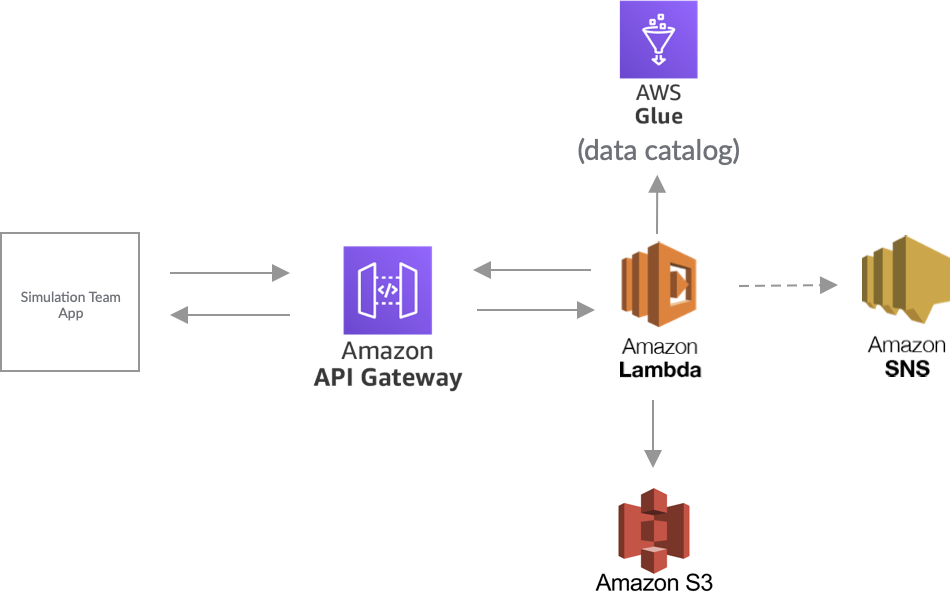
\includegraphics[width=0.8\linewidth]{images/Lambda.png}

\end{minipage}


\subsubsection{Metadata cataloguing}
\subparagraph{AWS Glue}
AWS Glue \cite{aws-glue} is a fully managed ETL (extract, transform, and load) service that makes it simple and cost-effective to categorize data, clean it, enrich it, and move it reliably between various data stores and data streams. AWS Glue consists of a central metadata repository known as the AWS Glue Data Catalog, an ETL engine that automatically generates Python or Scala code, and a flexible scheduler that handles dependency resolution, job monitoring, and retries. AWS Glue is serverless, so there’s no infrastructure to set up or manage.

\subparagraph{How it works}When used for metadata cataloguing, AWS Glue handles essential tasks:
\begin{itemize}
    \item Discovers and catalogs metadata about data stores into a central catalog. Semi-structured data can be processed, such as clickstream or process logs.
    \item Populates the AWS Glue Data Catalog with table definitions from scheduled crawler programs. Crawlers call classifier logic to infer the schema, format, and data types of data. This metadata is stored as tables in the AWS Glue Data Catalog and used in the authoring process of the ETL jobs.
    \item Detects schema changes and adapts by preference.
\end{itemize}
The data is stored in a Data Catalog made up Databases and Tables (Metadata). Databases are used to organize metadata tables in the AWS Glue. When a table is defined in the AWS Glue Data Catalog, it is added to a database. A table can be in only one database. 

\subparagraph{What is a crawler and how do they work?}A table can be defined using a crawler. Running a crawler connects to one or more data stores, determines the data structures, and writes tables into the Data Catalog. The crawler uses built-in or custom classifiers to recognize the structure of the data. A crawler can be ran on a schedule. To be noted that this is not the only way for creating tables, as the AWS Glue console can be used to manually create a table in the AWS Glue Data Catalog, or by using the CreateTable operation in the AWS Glue API. \cite{aws-crawlers}
\begin{itemize}
    \item A crawler runs any chosen custom classifier to infer the format and schema of your data. As the ingested data comes as HL7 FHIR messages through the RESTful endpoint, a custom classifier will be needed.
    \item The crawler connects to the data store. Some data stores require connection properties for crawler access.
    \item The inferred schema is created for the data.
    \item The crawler writes metadata to the Data Catalog. A table definition contains metadata about the data in the data store. The table is written to a database, which is a container of tables in the Data Catalog. Attributes of a table include classification, which is a label created by the classifier that inferred the table schema.
    \item If the crawler runs more than once, perhaps on a schedule, it looks for new or changed files or tables in the data store. The output of the crawler includes new tables and partitions found since a previous run.
\end{itemize}
\begin{figure}[h!]
	\centering
	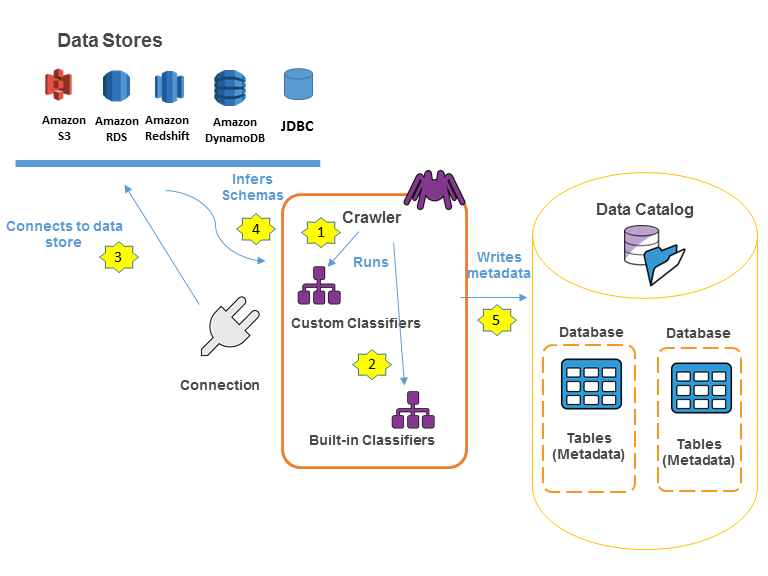
\includegraphics[width=0.9\linewidth]{images/PopulateCatalog-overview.png}
	\caption*{Example: General workflow for how a crawler populates the AWS Glue Data Catalog}
\end{figure}
\subparagraph{DataBrew}
This is a recently launched tool from AWS. It is not required for the completion of our project, but it can prove very useful in future development and extension of the project. \\ \\
AWS Glue DataBrew is a visual data preparation tool that enables users to clean and normalize data without writing any code. Using DataBrew helps reduce the time it takes to prepare data for analytics and machine learning (ML) by up to 80 percent, compared to custom developed data preparation. \\ \\
With the intuitive DataBrew interface, raw data can be interactively discovered, visualized, cleaned, and transformed. DataBrew makes smart suggestions that help to identify data quality issues that can be difficult to find and time-consuming to fix. The transformation steps can be saved in a recipe, which can be updated or reused later with other datasets, and deploy on a continuing basis. \cite{aws-databrew}
\begin{figure}[h!]
	\centering
	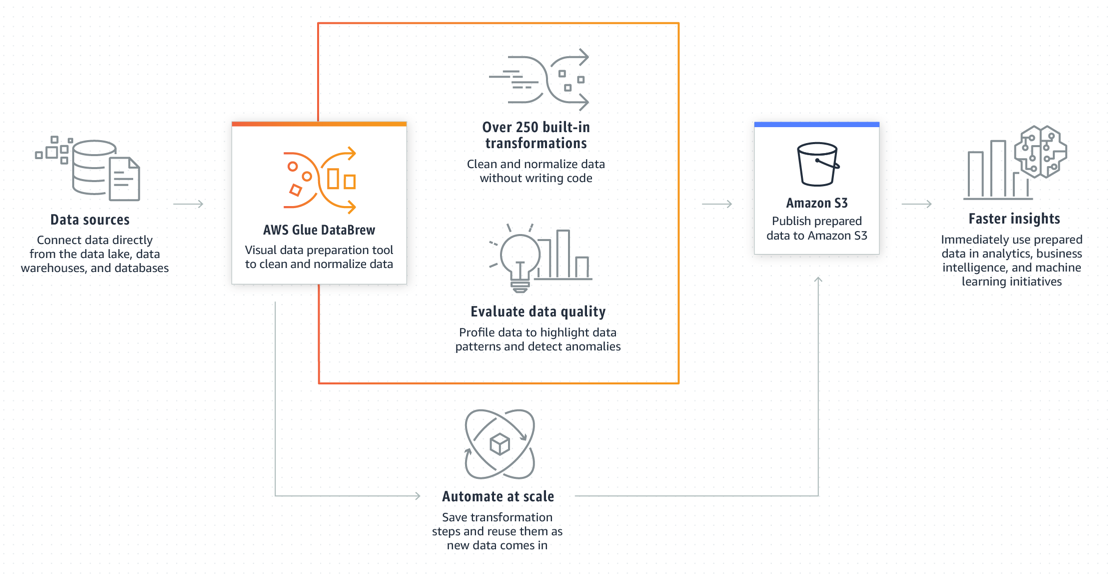
\includegraphics[width=0.9\linewidth]{images/databrew-overview-diagram.png}
	\caption*{Example: How DataBrew works at a high level}
\end{figure}

\subsubsection{Schema-less object store}
\paragraph{S3}
AWS Simple Storage Service (S3) \cite{S3} is an object storage service that offers industry-leading scalability, availability, security, and performance. S3 offers a range of storage classes including S3 Intelligent-Tiering for data with unknown or changing access patterns and S3 Glacier for long-term archive and digital preservation. S3 also offers capabilities to manage data throughout its lifecycle. \\ \\
S3 can use the AWS Global Infrastructure to be flexible and take advantage of the conceptually infinite scalability of the cloud. This gives the ability to instantly scale up or down the number of resources according to the application and user needs while reducing the cost. \\ \\
S3 can allow lots of access to shared data sets. S3 Access Point simplifies managing data access at scale for these applications. Access points are unique hostnames that customers create to enforce distinct permissions and network controls for any request made through the access point from applications. Any access point can be restricted to a VPC to firewall S3 data access within a private network. \\
\paragraph{S3 Glacier}
S3 Glacier\cite{S3-glacier} is a secure, durable, and low-cost storage class for data archiving. It provides three retrieval options that range from minutes to hours. There are two options to upload objects either directly or use S3 Lifecycle policies to transfer data between any of the S3 Storage Classes for active data. S3 Glacier stores data for as little as £0.003 per gigabyte per month.
\paragraph{Lifecycle Management}
To manage when objects are deleted or moved to and from a different storage class while being stored cost-effectively throughout their lifecycle, you can configure their S3 Lifecycle\cite{S3-lifecycle}. An S3 Lifecycle configuration is a set of rules that define actions that S3 applies to a group of objects. There are two types of actions:
\begin{itemize}
  \item Transition actions—Define when objects transition to another storage class (S3 Storage and Reduced Redundancy). An example might be transition objects to the S3 Standard-IA storage class 30 days after they are created, or archive objects to the S3 Glacier storage class one year after creating them. There are costs associated with the lifecycle transition requests. 
  \item Expiration actions—Define when objects expire. S3 automatically deletes the expired objects as defined. The lifecycle expiration costs depend on when you choose to expire objects. 
  \end{itemize}
\paragraph{Intelligent Tiering}
S3 Intelligent-Tiering \cite{S3-storage-classes} is an S3 storage class designed to optimize storage costs by automatically moving data to the most cost-effective access tier, without operational overhead.\\ \\
It works by storing objects in four access tiers: two low latency access tiers optimized for frequent and infrequent access and two opt-in archive access tiers designed for asynchronous access that are optimized for rare access (archive, and deep archive access).\\
\begin{figure}[h!]
   	\centering
   	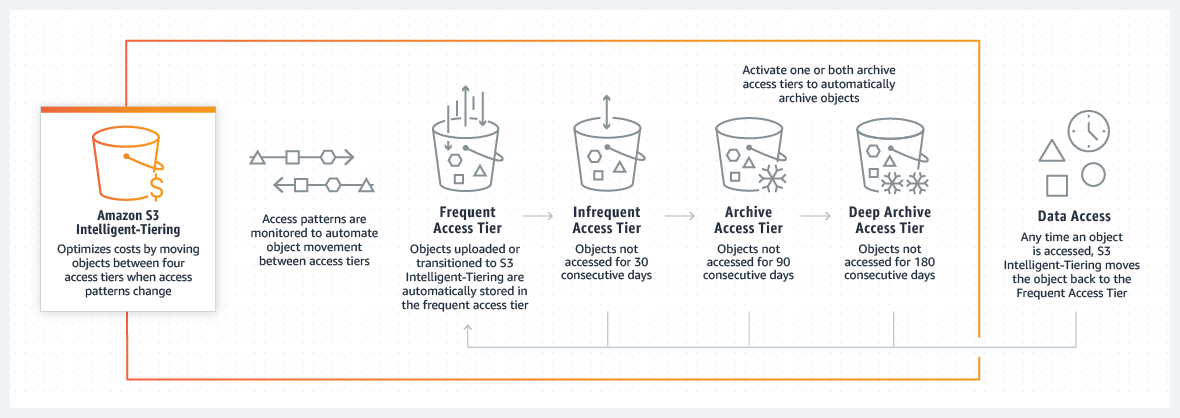
\includegraphics[width=1\linewidth]{images/S3-Intelligent-Tiering.png}	
\end{figure} \\
There are no retrieval fees when using the S3 Intelligent-Tiering storage class, and no additional tiering fees when objects are moved between access tiers within S3 Intelligent-Tiering. It is designed for durability of 99.999999999\% of objects across multiple Availability Zones and for 99.9\% availability over a given year.
\paragraph{Encyption} The encryption for Amazon S3 is explained in section 4.5. 

\newpage
\subsection{Data warehousing}
Data warehouses will be used in our project to store data that has been structured and cleansed from the data lake. This format lets us query the data so we can produce useful analytics and reports to return to the user.
\\
We will be using cloud-based data warehouses compared to on-premise warehouses because you do not have to purchase or maintain physical hardware, it is quicker and cheaper to initialise and scale, and can usually perform analytics queries much faster.
\paragraph{Options}There are many options to go with when it comes to cloud-based data warehouses.\cite{data-warehouse-comparisons}
\begin{itemize}
	\item \textbf{Google BigQuery} is a serverless architecture meaning resource management decisions are hidden from the user. Allows for the stream of data to the data warehouse. It uses the Dremel query execution engine which uses massively parallel processing (MPP) of querying to scan data in the Clossus file management system which uses clusters.
	\item \textbf{Snowflake} is a hybrid of traditional shared-disk database architectures and shared-nothing database architectures. Snowflake uses a central data repository for persisted data that is accessible from all compute nodes in the data warehouse. Snowflake also processes queries using MPP compute clusters.
	\item \textbf{AWS Redshift}\cite{redshift-architecture} uses traditional data warehouse approach.
\end{itemize}

\begin{figure}[h!]
   	\centering
   	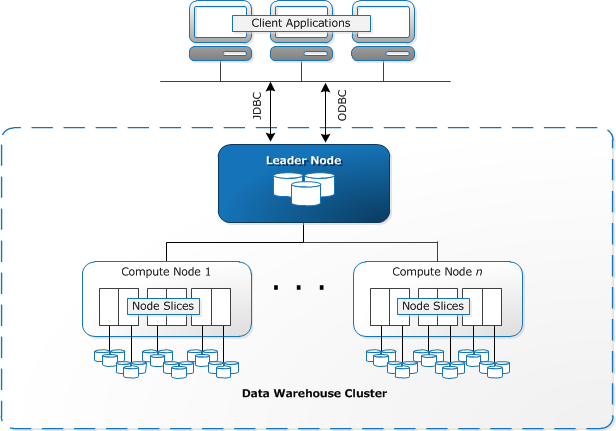
\includegraphics[width=0.7\linewidth]{images/Redshift-Architecture.png}	
   \end{figure}
Clusters are the core component of Redshift. If a cluster is provisioned with two or more compute nodes, an additional leader node coordinates the compute nodes and handles external communication. Client applications interact directly with the leader node only.\\
It parses and develops parallel execution plans to carry out database operations (results of queries). The leader node compiles code, distributes the compiled code to the compute nodes, and assigns a portion of the data to each compute node. It can increase the compute capacity and storage capacity of a cluster by increasing the number of nodes, upgrading the node type, or both.\\

\paragraph{Solution}For our project, we will be choosing Redshift firstly as it strongly focuses on the security of the data this is a major factor when we are dealing with personal data (\hyperref[sec:secure_access]{Section 4.5.1} discusses how Amazon Redshift uses encryption). Secondly, it is the cheapest as Redshift is the leader in being cost-efficient as it uses pay-as-you-go pricing so you only pay for what we will use. If we are using other AWS services, there will be a lot of support and documentation on the implantation and maintenance of the system. Other reasons include its highly scalable, easy to manage and has the best performance.\cite{redshift-benefits} 
\subsubsection{Federated querying}
Federated querying allows you to query data from multiple sources with different storage types to provide a solution. It will be used in our project to query from the data warehouse, remote sources, live data and straight from the data lake. Federated querying can remove the reliance on complex extract, transform, load (ETL) pipelines when loading data into the data storages.
\\ \\
An Example of Federate Querying with Amazon Redshift \cite{federate-queries} you can integrate queries from Redshift on live data in external databases with queries across your Redshift and S3 environments. Federated queries can work with external databases in AWS RDS and AWS Aurora. AWS Athena is a serverless SQL querying service for S3 that is also cost efficient and automatically scalable.
\subsubsection{Common models}
Common data warehouse models \cite{data-modelling} include virtual warehousing, data mart model and enterprise data warehouse model.
\\
We will be using the data mart model as it is used for business-line specific reporting and analysis. In this model, data is aggregated from a range of source systems relevant to a specific area. The data mart will then be used by the analytics team.
\subsubsection{Business Intelligence}
Furthermore, Redshift can create the data models for use in live Business Intelligence (\texttt{BI}) tools like visualisation dashboards and other high level business insights. This is compatible with many popular BI tools like Tableau, PowerBI and AWS QuickSight.

\newpage
\subsection{ETL \& data marts}
\begin{figure}[h!]
	\centering
	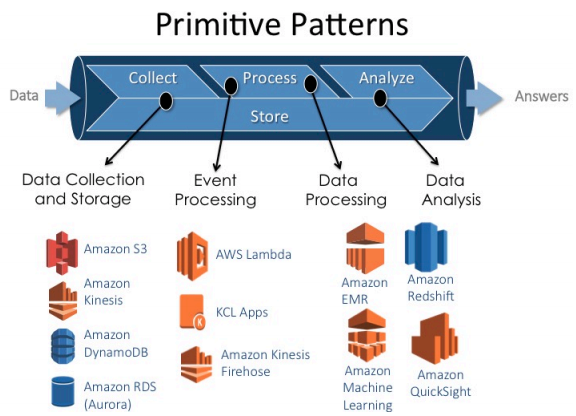
\includegraphics[width=0.8\linewidth]{images/AWSAnalyticsPipeline.png}
	\cite{aws-warehousing}
\end{figure}
\subsubsection{EMR cluster}
AWS Elastic MapReduce (\texttt{EMR}) is a service for running big data frameworks such as Apache Spark, Hive and Presto. It enables you to run petabyte-scale analysis at less than half the cost of on-premises solutions and over 3x the speed compared with standard Spark. It is easy to scale up and down and only pay per second of the instances used. It also provides Notebooks (based on Jupyter) for developers to work with and have all the heavy lifting taken care of with up to date dependencies. Encryption can be implemented with AWS KMS or customer-managed keys, for strong in-transit and at-rest encryption. IAM is used to create access controls for databases, tables and columns. \cite{aws-emr}
\subsubsection{Scheduling}
ETL workloads can be automated using EMR with AWS Data Pipeline for movement of complex data processing workloads that are fault tolerant by ensuring availability, managing dependencies, retrying failures or timeouts or creating a failure notification system. As expected, this service is also easy to use, flexible / scalable, cheap and extremely reliable. This could be used to move on-premise data silos into the lake if desired.
\begin{figure}[h!]
	\centering
	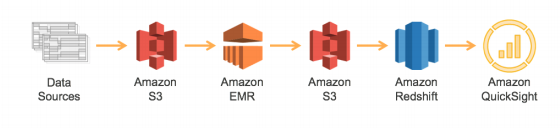
\includegraphics[width=0.8\linewidth]{images/AWSWorkflow.png}
	\cite{aws-warehousing}
\end{figure}

\subsection{Secure access}
\label{sec:secure_access}

\subsubsection{Encryption}

When data is received, it will require a key to encrypt the data. This key is typically generated by a key manager. When data is being retrieved or queried it will then use the same key to decrypt the data to be used.
\\ \\
A key manager is used to generate, exchange, use, replace and delete cryptographic keys. It's able to deal with asymmetric and symmetric keys. Some key managers encrypt keys after generation to add another layer of security.
\\ \\
Client-side encryption is an alternative option to encrypt the data locally in the application before it gets to the lake. This means the lake is not involved in the cryptographic process of the data, as the application will use its own encryption key which the lake cannot access. This is beneficial for the users as it provides them peace of mind.
\paragraph{Solutions} 
Cloud computing services \textit{Azure}, \textit{GCP} and \textit{AWS} all provide options for client and server-side encryption.
\\ \\
We will be looking at AWS Simple Storage Service (\texttt{S3}) \cite{encryption-in-s3}, AWS Redshift \cite{encryption-in-redshift} and AWS Key Management Service (\texttt{KMS}) for an example of the implementation of encryption.
\subparagraph{AWS S3}
Server-side encryption uses three different modes of server-side encryption: SSE-S3, SSE-C, or SSE-KMS. The following will be an example of SSE-KMS.
\\ \\ 
SSE-KMS enables the choice of a customer-managed Customer Master Key (\texttt{CMK}) or the AWS managed CMK for Amazon S3 in the account. AWS KMS and Amazon S3 perform the following actions on encryption:
\begin{itemize}
  \item Amazon S3 requests a plaintext data key and a copy of the key encrypted under the specified CMK.
  \item AWS KMS generates a data key, encrypts it under the CMK and sends both the plaintext data key and the encrypted data key to Amazon S3.
  \item Amazon S3 encrypts the data using the data key and removes the plaintext key from memory as soon as possible after use.
  \item Amazon S3 stores the encrypted data key as metadata with the encrypted data.
\end{itemize}

Amazon S3 and AWS KMS perform the following actions when data is requested to be decrypted:
\begin{itemize}
    \item Amazon S3 sends the encrypted data key to AWS KMS.
    \item AWS KMS decrypts the key by using the same CMK and returns the plaintext data key to Amazon S3.
    \item Amazon S3 decrypts the ciphertext and removes the plaintext data key from memory as soon as possible.
\end{itemize}

Client-Side Encryption with AWS can use Amazon S3 Encryption Client in the AWS SDK of an application to encrypt objects and upload them to Amazon S3. This method ensures its security as it passes to the Amazon S3 service. The Amazon S3 service receives the encrypted data; it does not play a role in encrypting or decrypting it.

\subparagraph{AWS Redshift}
Amazon Redshift uses a four-tier, key-based architecture for encryption. The architecture consists of data encryption keys, a database key, a cluster key and a master key.
\\
\begin{enumerate}
	\item Data encryption keys encrypt data blocks in the cluster. Each data block is assigned a randomly generated 256-bit AES key. These keys are encrypted by using the database key for the cluster.
	\item The database key encrypts data encryption keys in the cluster. The database key is a randomly generated AES-256 key. It is stored on disk in a separate network from the Redshift cluster and passed to the cluster across a secure channel.
	\item The cluster key encrypts the database key for the Redshift cluster.  KMS, AWS CloudHSM, or an external hardware security module (\texttt{HSM}) can be used to manage the cluster key.
	\item The master key encrypts the cluster key. KMS CMK can be used as the master key for Redshift.
\end{enumerate}


\subparagraph{AWS KMS}

AWS Key Management Service (\texttt{KMS}) allows you to create and manage cryptographic keys and control their use across a wide range of AWS services and in the applications. AWS KMS uses hardware security modules (\texttt{HSM}s) that have been validated under FIPS 140-2, to protect keys. AWS KMS is integrated with AWS CloudTrail to provide logs of all key usage to help meet applicable regulatory and compliance needs. \cite{aws-kms}
\\ \\
S3 handles the process of Server-Side Encryption (\texttt{SSE}) \cite{encryption-with-aws-kms}
\begin{itemize}
    \item When an object is uploaded into S3 and specified SSE, a unique 256-bit key (a data key) is generated and the data is encrypted using that key with AES-256.
    \item The data key is then encrypted using a master key, which S3 retrieves from KMS using the master key ID that was supplied.
    \item The encrypted data key is then stored with the encrypted data in the S3 bucket.
\end{itemize}

\newpage

\subsubsection{IAM}
\paragraph{Concept}
Identity and Access management (\texttt{IAM}) is used to make sure authorised users have the right to services while preventing access to non-authorised users (guaranteeing secure access). It does this by defining and managing the roles, the access privileges of individual users and the circumstance users are granted those privileges.
\\ \\
IAM allows access management over computing, storage, database and application services. It gives one identity per individual. Once that identity has been introduced, it must be maintained, modified and monitored throughout each user’s access lifecycle. \cite{iam}
\paragraph{Solution}
We will be examining AWS IAM \cite{aws-iam}. IAM is a feature of an AWS account offered at no additional charge. 
\\ \\
The use cases of AWS IAM include finite-grained access control to AWS resources, multi-factor authentication for high privilege users, analysis of access across the AWS environment and ability to integrate with the corporate directly (integration of current IAM system). 
\subparagraph{How it works}
AWS IAM allows us to:
\begin{itemize}
    \item Manage IAM users and their access –  Create users in IAM, assign them individual security credentials (access keys, passwords and multi-factor authentication devices), or request temporary security credentials to provide users access to AWS services and resources. Manage permissions in order to control which operations a user can perform.
    \item Manage IAM roles and their permissions – Create roles in IAM and manage permissions to control which operations can be performed by the entity, or AWS service, that assumes the role. Define which entity can assume the role. In addition, you can use service-linked roles to delegate permissions to AWS services that create and manage AWS resources automatically.
    \item Manage federated users and their permissions – Enable identity federation to allow existing identities (users, groups and roles) in the enterprise to access the AWS Management Console, call AWS APIs and access resources, without the need to create an IAM user for each identity. Enable the use of any identity management solution that supports SAML 2.0.
\end{itemize}

\newpage
\subsubsection{Logging}
\paragraph{Concept}
Using logs to monitor the use of the system provides security to check for violations and unpredicted behaviour from users and the system. Analysing, searching and filtering logs discovers and alerts these incidents. It enables access to historic information for debugging and forensic investigations. \cite{logs}
\paragraph{Examples}
The example which will show the use of logs is AWS CloudWatch. CloudWatch can be used to monitor, store and access the log files from AWS Services.
\\ \\
CloudWatch enables the centralization of the logs from all over the systems, applications and AWS services that are used, in a single, highly scalable service. You can then easily view them, search them for specific error codes or patterns, filter them based on specific fields, or archive them securely for future analysis. \cite{aws-cloudwatch}
\subparagraph{Features}
\begin{itemize}
	\item Querying – CloudWatch Insights can be used to interactively search and analyse log data. 
	\item Monitor AWS CloudTrail Events – You can create alarms in CloudWatch and receive notifications of particular API activity as captured by CloudTrail and use the notification to perform troubleshooting.
	\item Log Retention – By default, logs are kept indefinitely and never expire. You can adjust the retention policy for each log group, keeping the indefinite retention, or choosing a retention period between 10 years and one day.
	\item Archive Log Data – CloudWatch Logs can be used to store log data in highly durable storage. The CloudWatch Logs agent makes it easy to quickly send both rotated and non-rotated log data off of a host and into the log service. You can then access the raw log data when needed.
\end{itemize}

\newpage
\subsection{Network}
\label{sec:network}
\begin{figure}[h!]
	\centering
	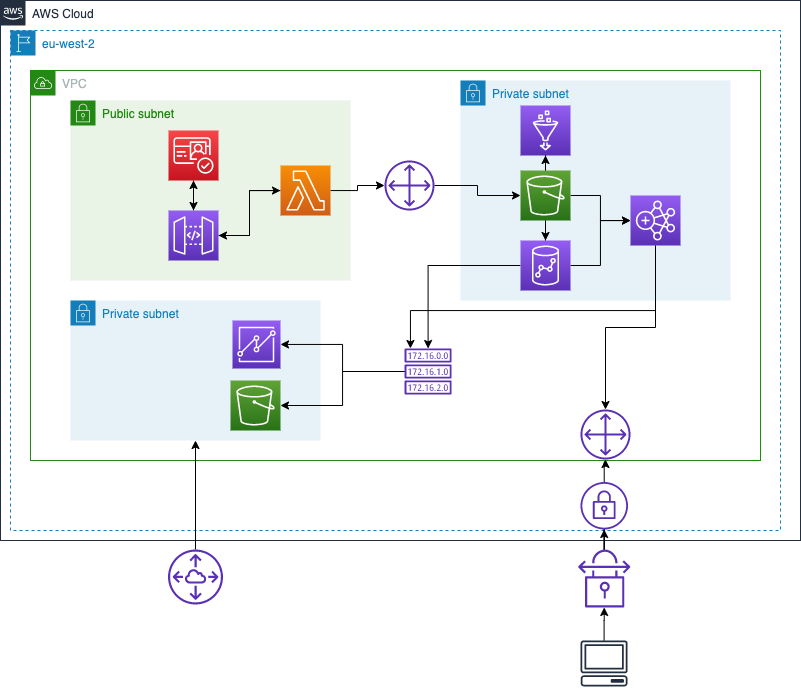
\includegraphics[width=0.62\linewidth]{images/Network.png}
\end{figure}
\subsubsection{Public subnet (API)}
The client API is accessible over the WAN on all IPv4 and IPv6 addresses (0.0.0.0/0, ::/0). In future versions, it may be decided to make this a private network though. In front of the Lambda sits the API Gateway, forwarding requests to and fro. Lambdas may not be directly invoked. The Lambda only has the following IAM permissions: \texttt{PutObject} and \texttt{UploadPart}. This would ideally be replicated across at least two availability zones in the region so that downtime is prevented.
\subsubsection{Private subnet A (Data Lake)}
The lake itself contains the S3 bucket, Glue instance, Redshift instance and EMR cluster. These are needed for all the ETL jobs and federated querying. Optionally, an AWS Athena instance could be added here for SQL querying across the lake. The EMR cluster can be accessed securely via a VPN client connection.
\subsubsection{Private subnet B (Trusted Research Environment)}
Once big data tasks are run across the lake to cleanse and prepare data marts, they are written to an S3 bucket inside a private subnet for use in the analytics environment. Additionally, Redshift can be used for warehousing the data marts and provide Business Intelligence tools with data. An example of AWS QuickSight has been included here, but most BI tools like Tableau are compatible with S3 anyway and if not, then Redshift solves that problem by providing data warehousing so that models are there for querying.
\subsubsection{VPC peering}
Private subnet B, or the Trusted Research Environment (hereinafter "\texttt{TRE}"), is accessible to the Data Analytics team via a VPC peering connection. This assumes the VPCs are held in the same AWS Organization account, ensuring IAM roles can be used across VPCs.

\iffalse
\subsection{Streaming data (Optional)}
\subsubsection{Kinesis Firehose}
\subsubsection{Medical IoT}
\subsubsection{Wearables / sensors}
\subsubsection{EHR}
\subsubsection{Digital medical imagery}
\subsubsection{Real-time analytics}
\fi

\subsection{Extensible}
\subsubsection{Databricks integration}
\begin{figure}[h!]
	\centering
	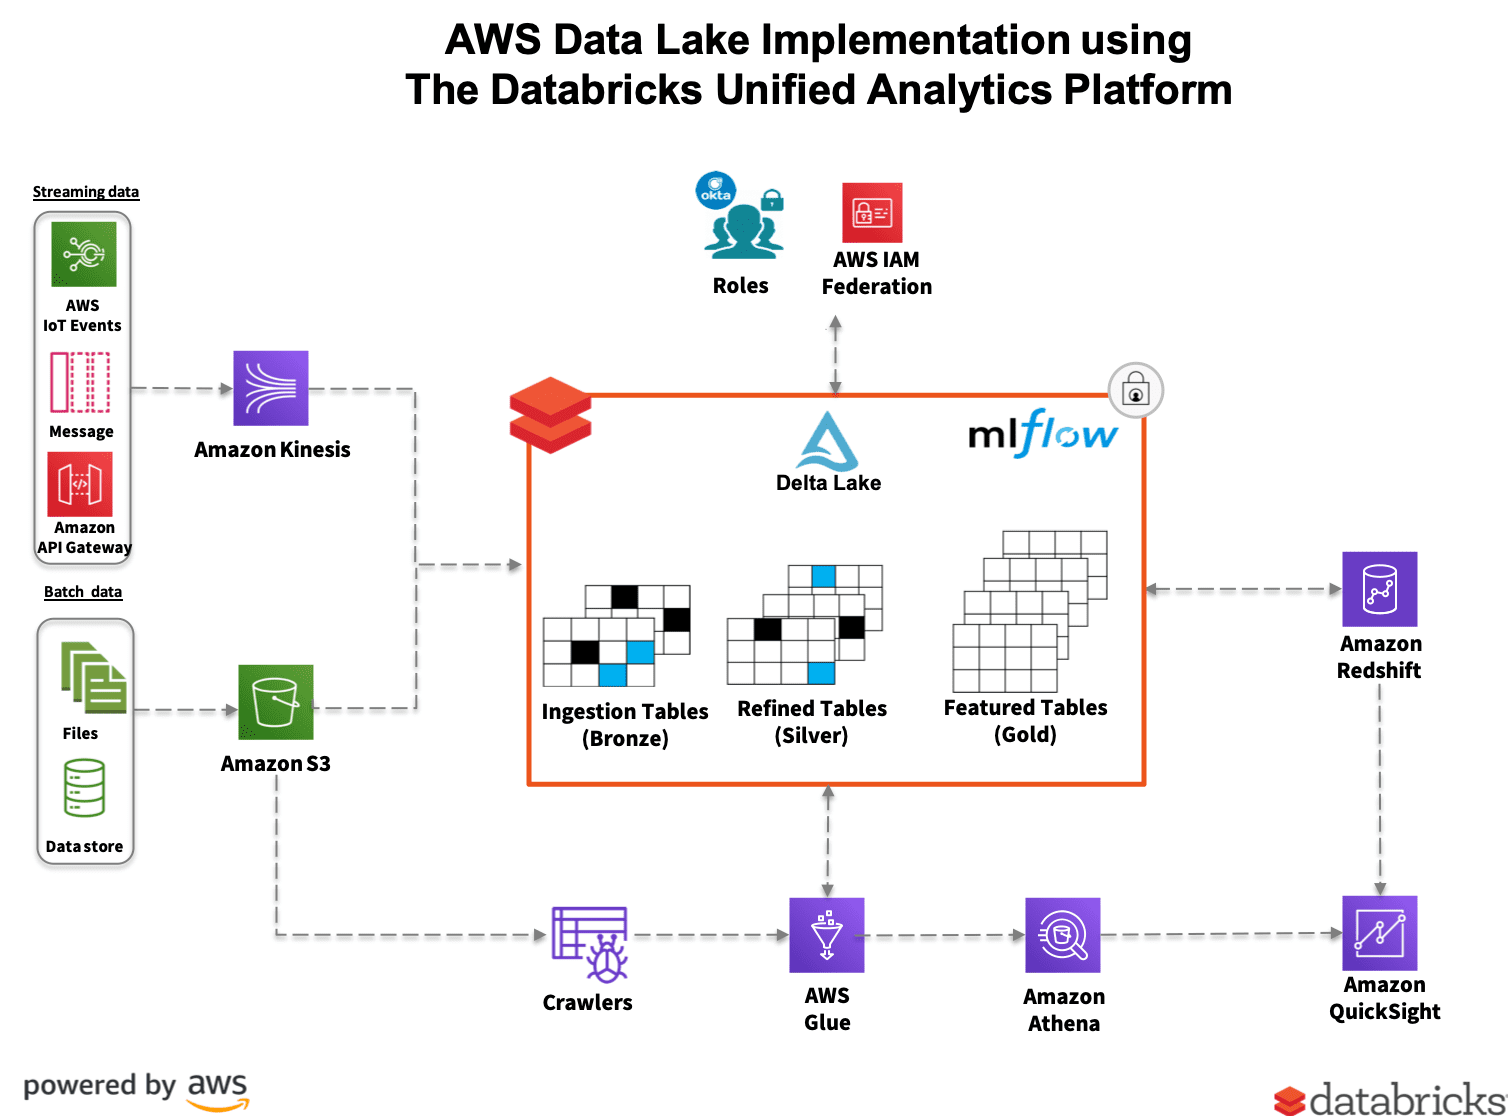
\includegraphics[width=0.9\linewidth]{images/AWS-Data-Lake-Architecture-light-BG.png}
\end{figure}
\paragraph{What is Databricks?} DataBricks is a start-up offering a Unified Data Analytics Platform, one cloud platform for massive scale data engineering and collaborative data science. The platform is designed to integrate AWS and Azure solutions to create one reliable and scalable data lake
for all analytics, create a collaborative workspace for data and Machine Learning teams and deploy one platform for data science, Machine Learning, and analytics. \cite{databricks}
\\ \\
In the further development of the project by the NHS Digital teams, Databricks can be easily integrated to offer extraordinary data analytics opportunities, beyond the initial intended purpose of the project.
\paragraph{Integration}
\begin{itemize}
    \item \textbf{Amazon Redshift} Databricks can read data securely from Redshift and integrate it with other datasets. With Delta Lake, Databricks can make that data into simplified and reliable data pipelines using optimized cluster resources. Data can then be used for machine learning in Databricks, or put back into Redshift for data warehouse workloads.
    \item \textbf{AWS Glue Integration} Being a Apache compatible Hive serverless metastore, AWS Glue integration offers several benefits such as simplified manageability by using the same AWS Glue catalog across multiple Databricks workspaces or simplified integrated security using IAM Credntial Passthrough for metadata in AWS Glue.
    \item \textbf{Amazon SageMaker} Databricks is integrated with Amazon SageMaker using MLflow to enable distribution of machine learning models. Databricks is used to build collaborative ML models and train them at scale. The deployment enables real-time model serving and REST API integration.
    \item \textbf{Automated, High Scale Data Pipelines} Created automated data pipelines at scale that minimize cost with features such as auto-clustering and spot pricing. Using Delta Lake, you can scale up to the largest datasets, with high velocity data providing constant updates, instantly available for analytics.
	\item \textbf{Delta Lake} Delta Lake is an open source project with the Linux Foundation. Data is stored in the open Apache Parquet format, allowing data to be read by any compatible reader. It offers integration for existing Amazon S3 storage service. Delta Lake adds a storage layer to data lakes to manage data quality, ensuring data lakes contain only high quality data for consumers. The Delta Lake transaction log records details about every change made to data, providing a full history of changes, for compliance, audit, and reproduction.
\end{itemize}

\subsubsection{Multi-vendor}

\section{Development Testing}
\subsection{Local environment}

\subsubsection{API}
\paragraph{Serverless}
The Serverless Framework enables developers to run an emulated environment locally instead of needing to deploy that serverless app for testing. This comes with over 1,000 plugins that can emulate services such as AWS Lambda and API Gateway. 
\\ \\
Therefore, developers are expected to build and test their code locally with identical behaviour to that of the deployment environment. As any microservice can be done in a number of languages, it is not decided which framework is chosen for unit tests of those.
\paragraph{Postman}

Postman is a very popular tool used by developers that want to conveniently test and build APIs in a collaborative way.
\\ \\
As we are implementing the OpenAPI specification, Postman enables the import of Swagger files to automatically generate a Postman environment. This makes developer on-boarding much easier as versioned mock endpoints and documentation are hosted for us as part of the DevOps deployment. It enables tests to be written as well (JavaScript), but we may opt to use a different RESTful testing framework such as REST-assured (Java).

\subsubsection{Infrastructure}
The shared infrastructure differs from that of the application infrastructure (in this case referring to the serverless API). The shared infrastructure can be built, updated, reverted and destroyed easily using the Terraform command-line tools (\texttt{cli}). Terraform formats and validates your plan before applying it, so writing unit tests around the migration itself doesn't make sense in this context. What does make sense is testing the enforcement of user-defined standards. This can be written with Terraform Validate (Python) or Terratest (Go). Furthermore, compliance controls could be generated with Chef InSpec profiles ("Compliance-as-Code").

\paragraph{Docker}
To achieve consistency across developers' local machines and avoid headaches, Docker containers will be used for the local development environments.

\paragraph{Terraform}
Terraform workspaces are utilised to isolate development, staging and production environments. It also gives developers the option to work on their own accounts without breaking global state. However, a global state backend will be configured with S3 and a state lock with DynamoDB to enable a team to work on the same infrastructure.

\subsection{DevOps}
\begin{figure}[h!]
	\centering
	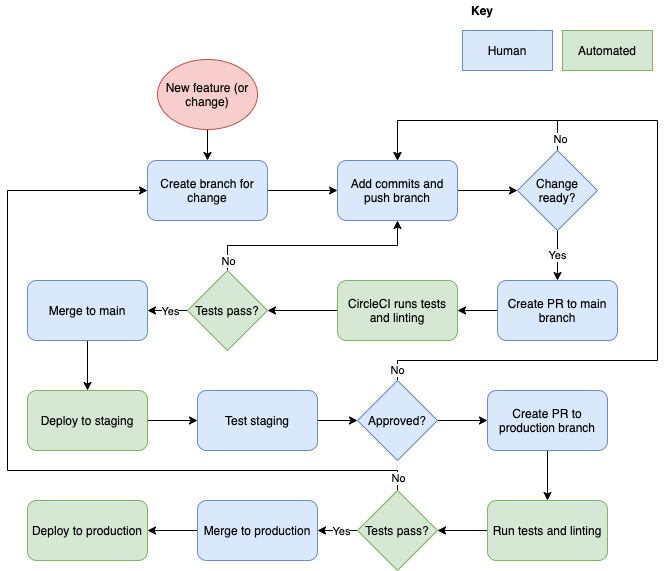
\includegraphics[width=0.9\linewidth]{images/DevOpsWorkflow.png}	
\end{figure}

\subsubsection{GitHub}
The git repository is hosted on GitHub in the custody of the organisation. However, the repository will be MIT licensed.
\subsubsection{CircleCI}
The Continuous Integration \& Continuous Delivery pipelines are run by CircleCI servers. This decision was made by the university. Jenkins (self-hosted) would be preferred to reduce overall cost constraints and just generally to reduce vendor lock-in and improve security. The workflows of jobs are defined in a YAML configuration file. 
\subsubsection{Terraform}
Terraform handles the deployment by using the relevant APIs - in this case it will use the AWS API but may use any other providers as required - such as if we decided to integrate Azure or Google for a multi-vendor infrastructure.


\section{Release Testing}
\subsection{Staging}
\subsection{Production}


\newpage
\printbibliography

\end{document}
